\documentclass[12pt]{article}
\usepackage[]{graphicx}
\usepackage[]{geometry}
\usepackage[]{amsmath}
\usepackage[]{amssymb}
\usepackage[table]{xcolor}
\usepackage{listings}
\usepackage{array}
\newcolumntype{P}[1]{>{\centering\arraybackslash}m{#1}}
\setlength{\arrayrulewidth}{0.5mm}
\setlength{\tabcolsep}{10pt}
\usepackage{algpseudocode}
\usepackage{algorithm2e,caption}
\usepackage[nottoc,numbib]{tocbibind}
\usepackage{hyperref}
\usepackage[utf8]{inputenc}
\RestyleAlgo{ruled}
\usepackage{multirow}
\usepackage[labelformat=empty]{caption}
\hypersetup{
    colorlinks=true,
    linkcolor=blue,
    filecolor=magenta,      
    urlcolor=cyan,
    pdftitle={Overleaf Example},
    pdfpagemode=FullScreen,
    }

\urlstyle{same}
\usepackage{geometry}
 \geometry{
 a4paper,
 total={170mm,250mm},
 left=20mm,
 top=20mm,
 }
\SetKwComment{Comment}{/* }{ */}
\definecolor{codegreen}{rgb}{0,0.6,0}
\definecolor{codegray}{rgb}{0.5,0.5,0.5}
\definecolor{codepurple}{rgb}{0.58,0,0.82}
\definecolor{backcolour}{rgb}{0.95,0.95,0.92}

\lstdefinestyle{mystyle}{
    backgroundcolor=\color{backcolour},   
    commentstyle=\color{codegreen},
    keywordstyle=\color{magenta},
    numberstyle=\tiny\color{codegray},
    stringstyle=\color{codepurple},
    basicstyle=\ttfamily\normalsize,
    breakatwhitespace=false,         
    breaklines=true,                 
    captionpos=t,                    
    keepspaces=true,                 
    numbers=left,                    
    numbersep=5pt,                  
    showspaces=false,                
    showstringspaces=false,
    showtabs=false,                  
    tabsize=2
}

\lstset{style=mystyle}


\title{\textbf{Software Systems Lab: OutLab \\ \LaTeX{}}}
\author{Name: Shubham Hazra\\Roll no: 210100143}
\date{\Large{September 4, 2022}}

\renewcommand*\contentsname{Lab 3 - SED and AWK}

\begin{document}

\vspace*{20em}
\begin{center}
    \huge 
    \textbf{Software Systems Lab: OutLab}\\
    \vspace*{1em}
    \textbf{\LaTeX{}}\\
    \large
    \vspace*{1em}
    Name: Shubham Hazra\\
    Roll no: 210100143\\
    \vspace*{1em}
    \LARGE
    August 30, 2022
\end{center}

\newpage

\tableofcontents
\newpage

\section{Introduction}
\vspace*{4em}
\begin{center}
    {\Large{\textbf{SED}}}
\end{center}
\fbox
{
\begin{minipage}{\textwidth}
    Sed is a stream editor. A stream editor is used to perform basic text 
    transformations on an input stream (a file or input from a pipeline). 
    While in some ways similar to an editor which permits scripted edits 
    (such as ed), sed works by making only one pass over the input(s), and is 
    consequently more efficient. But it is sed’s ability to filter text in a 
    pipeline which particularly distinguishes it from other types of editors.
    \\
    The basic syntax is:\\
    \emph{sed 'sed\_command' filename}\\
    For example:\\ To substitute a certain pattern1 with another pattern2 in a file:\\
    \emph{sed 's/pattern1/pattern2/' filename}
    \\
    To print k lines of a file:\\
    \emph{sed -n 'kp' filename}\\
    To delete k lines of a file:\\
    \emph{sed 'kd' filename}\\
    For inplace substitutions:\\
    \emph{sed -i 's/pattern1/pattern2/' filename} \cite{geeksforgeeks1}
\end{minipage}
}\\\\\\\\
\begin{center}
    {\Large{\textbf{AWK}}}
\end{center}
\fbox
{
\begin{minipage}{\textwidth}
    AWK (awk) is a domain-specific language designed for text processing and 
    typically used as a data extraction and reporting tool. Like sed and grep, 
    it is a filter, and is a standard feature of most Unix-like operating 
    systems.
    The AWK language is a data-driven scripting language consisting of a set of 
    actions to be taken against streams of textual data – either run directly on files
    or used as part of a pipeline – for purposes of extracting or transforming text, 
    such as producing formatted reports. The language extensively uses the string 
    datatype, associative arrays (that is, arrays indexed by key strings), and 
    regular expressions. While AWK has a limited intended application domain and was 
    especially designed to support one-liner programs, the language is Turing-
    complete.\\
    The basic syntax is:\\
    \emph{awk 'BEGIN\{\} \{\} END\{\}' filename}\\
    For example:\\
    To print contents of a file:\\
    \emph{awk '\{print\}' filename} \cite{geeksforgeeks}
\end{minipage}
}
\newpage
\setlength{\arrayrulewidth}{0.5mm}
\begin{center}
    \begin{table}
        \label{sedvsawk}
        \caption{\label{tab:sedvsawk}\textbf{\Large{SED vs AWK}}}
        \renewcommand{\arraystretch}{4}
        \rowcolors{1}{green!80!yellow!50}{green!70!yellow!40}
        \begin{tabular}{|P{0.45\textwidth}|P{0.45\textwidth}|}
            \hline
            \textbf{SED} & \textbf{AWK}
            \\ \hline
            A command line utility that parses and transforms text, using a simple
            , compact programming language & A command line utility designed for text
            processing that allows effective programs in the form of statements\\ 
            \hline
            Less powerful & More powerful and robust\\ 
            \hline
            Simple and limited & Complex and versatile\\
            \hline
        \end{tabular}
    \end{table}
\end{center}
\vspace*{1em}
In this lab I was required to write sed commands and awk scripts on bash for the 
various inlab and outlab problems. There were 3 inlab problems and 5 outlab problems.
However I am only going to cover one problem from the inlab and one from the outlab 
in this report.\\
The following are the methods I used to solve the problems:\\
\begin{itemize}
    \item InLab
    \begin{enumerate}
        \item Q1\_a :- awk
        \item Q1\_b :- awk
        \item Q2    :- awk
        \item Q3    :- sed
    \end{enumerate}
    \item OutLab
    \begin{enumerate}
        \item Q1 :- sed
        \item Q2 :- sed
        \item Q3 :- awk
        \item Q4 :- awk
        \item Q5 :- awk and sed
    \end{enumerate}
\end{itemize}

\newpage

\section{Inlab 3 - Q2}

\subsection{Problem Statement}
Create a function which takes in input a set of numbers from a text file 
in base 8+2*(line\_number\%3) 
and returns the same number in base 10. 
Note that the digits will be space separated on each line. 
For digits greater than 9, lowercase alphabets will be used.\\\\\\\\\\
\begin{figure*}[h]
    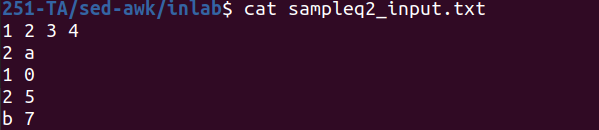
\includegraphics[width=\textwidth]{inlab3_sample_input.png}
    \caption[]{Sample Input}
\end{figure*}\\\\\\\\
\begin{figure*}[h]
    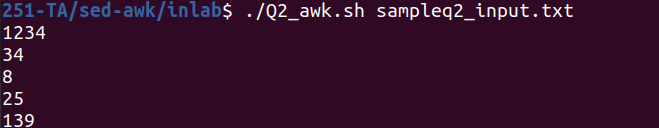
\includegraphics[width=\textwidth]{inlab3_sample_output.png}
    \caption[]{Sample Output}
\end{figure*}
\newpage

\subsection{Algorithm}
\vspace*{2em}
The algorithm that my code follows is:\\\\
\begin{algorithm*}
    \label{Q2}
    \caption{InLab - Q2}\label{alg:Q2}
    \While{read line}
    {
        $num\_digits \gets \textrm{number of fields(NF)}$\;
        \For{$i \gets 1 \textrm{ to } num\_digits$}
        {
            $digits[i-1] \gets \$i\textrm{(Value of that field)}$\;
            \Comment{digits gets 10 if value is a, 11 for b and 12 for c} 
        }
        $base \gets 8 + 2\cdot\textrm{NR(Number of row)\%}3$\;
        $sum \gets 0$\;
        \For{$i \gets 0 \textrm{ to } num\_digits-1$}
        {
            $sum \gets sum + digits[i]\cdot base^{(num\_digits-i-1)}$\;
        }
        print $sum$\;
    } 
\end{algorithm*}
\newpage

\subsection{Code}
\vspace*{2em}
The code that I wrote is:\\\\
References from : \cite{oreilly} \cite{unix} \cite{computerworld}\\\\
\begin{lstlisting}[language=bash, caption=InLab - Q2]
    #!/bin/bash

    awk '
    {
        num_digits=NF;
        for(i=1;i<=NF;i++)
        {
            if($i=="a")
            {digits[i-1]=10}
            else if($i=="b")
                    {digits[i-1]=11}
            else if($i=="c")
                    {digits[i-1]=12}
            else {digits[i-1]=$i}
        }
        base=8+2*(NR%3)
        sum=0;
        for(i=0;i<num_digits;i++)
        {
            mult=1;
            for(j=0; j<num_digits-i-1; j++)
            {
                mult=mult*base;
            }
            sum=sum+digits[i]*mult;
        }
        print sum
    }' $1 
\end{lstlisting}
\newpage

\subsection{Results}
\vspace*{1em}
The \textbf{input}, the \textbf{command} I ran and the \textbf{output} I got are:\\\\
\begin{figure*}[h]
    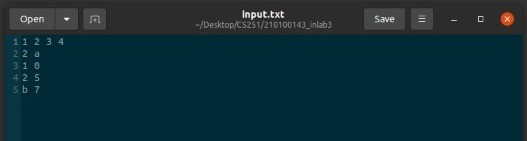
\includegraphics[width=\textwidth]{Q2_input.jpeg}
    \caption[]{Input}
\end{figure*}
\vspace*{1em}
\begin{figure*}[h]
    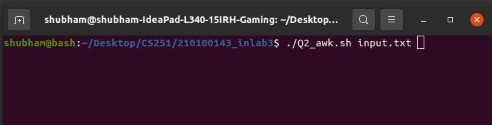
\includegraphics[width=\textwidth]{Q2_command.jpeg}
    \caption[]{Command}
\end{figure*}
\vspace*{1em}
\begin{figure*}[h]
    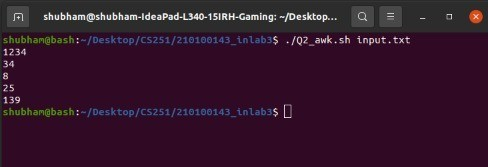
\includegraphics[width=\textwidth]{Q2_output.jpeg}
    \caption[]{Output}
\end{figure*}
\newpage

\section{Outlab 3 - Q4}

\subsection{Problem Statement}
Your task for this question is to perform addition of two numbers and 
write the result to file for each test case.\\\\
\textbf{Sample Input:}\\\\
1
\\
10 2
\\
9 9 9
\\
1 0 0
\\
\\
\textbf{Input description:}
\\
First line of the file indicates the number of test cases.
Second Line gives the base of the input and output separated by spaces. 
The next two lines of each test case have two numbers. 
The digits of the numbers are space separated. 
The base is guaranteed to be less than or equal 16.
\\\\
\textbf{Expected output for the above input:}
\\\\
1 0 0 0 1 0 0 1 0 1 1
\\\\
\textbf{Output description:}
\\
The digits in each result should be space separated. 
Each line should contain only one result.\\\\
Write the bash script q4.sh that takes two text files, one containing input and 
other to write the output. 
Make use of \textbf{awk} (mandatory!) to solve the task.
\\\\\\\\\\\\
\subsection{Algorithm}
The following algorithm was written by using the algorithm2e package which is able 
to make the most good looking algorithms, however this package does not allow page
breaks and the following algorithm is too big to fit in one page with the section
heading so I removed the page break from the above section and added this algorithm 
section to the same page so the algorithm is able to render fully in the page below.\\
\\\\\\\\
The algorithm that my code follows is:\\\\
\begin{algorithm*}
    \label{Q4}
    \caption{OutLab - Q4}\label{alg:Q4}
    \While{read line}
    {
        \If{NR==1}
        {
            testcases=\$1\;
        }
        \If{NR\%3==2}
        {
            input\_base=\$1\;
			output\_base=\$2\;
        }
        \If{NR\%3==0}
        {
            num\_digits1=NF\;
            \For{$i \gets 1 \textrm{ to } num\_digits1$}
            {
                $digits1[i] \gets \$i\textrm{(Value of that field)}$\;
                \Comment{digits gets 10 if value is a, 11 for b and so on till 15 for f} 
            }
            $num1 \gets 0$\;
            \For{$i \gets 0 \textrm{ to } num\_digits1-1$}
            {
                $num1 \gets num1 + digits[i]\cdot input\_base^{(num\_digits1-i-1)}$\;
            }
        }
        \If{NR\%3==0 and NR!=1}
        {
            num\_digits2=NF\;
            \For{$i \gets 1 \textrm{ to } num\_digits2$}
            {
                $digits2[i] \gets \$i\textrm{(Value of that field)}$\;
                \Comment{digits gets 10 if value is a, 11 for b and so on till 15 for f} 
            }
            $num2 \gets 0$\;
            \For{$i \gets 0 \textrm{ to } num\_digits2-1$}
            {
                $num2 \gets num2 + digits[i]\cdot input\_base^{(num\_digits2-i-1)}$\;
            }
            $sum \gets num1 + num2$\;
            num\_digits=0\;
            i=0\;
			\While{$sum > 0$}
			{	
				digits[i]=int(sum\%output\_base)\;
				sum=int(sum/output\_base)\;
				num\_digits++\;
				i++\;
			}
            \For{$i \gets num\_digits-1 \textrm{ to } 0$}
            {
                print digits[i]
            }
            print new line
        }

    } 
\end{algorithm*}
\newpage

\subsection{Code}
The code that I wrote is:\\
References from : \cite{oreilly} \cite{unix} \cite{computerworld} \cite{unix-stackexchange}
\begin{lstlisting}[language=bash, caption=OutLab - Q4]
    #!/bin/bash

    awk '{
        if(NR==1)
        {
            testcases=$1
        }
        if(NR%3==2)
        {	
            input_base=$1;
            output_base=$2;
        }
        if(NR%3==0)
        {
            num_digits1=NF;
            for(i=1;i<=NF;i++)
            {
                if($i>=0 && $i<=9)
                {digits1[i-1]=$i}
                else if($i=="a")
                {digits1[i-1]=10}
                else if($i=="b")
                {digits1[i-1]=11}
                else if($i=="c")
                {digits1[i-1]=12}
                else if($i=="d")
                {digits1[i-1]=13}
                else if($i=="e")
                {digits1[i-1]=14}
                else if($i=="f")
                {digits1[i-1]=15}
                else
                {digits1[i-1]=$i}    
            }
            num1=0;
            for(i=0;i<num_digits1;i++)
            {
                mult=1;
                for(j=0; j<num_digits1-i-1; j++){
                mult=mult*input_base;
                }
                num1=num1+digits1[i]*mult;
            }
            }
            if(NR%3==1 && NR!=1)
            {
                num_digits2=NF;
                for(i=1;i<=NF;i++)
                {
                    if($i>=0 && $i<=9)
                    {digits2[i-1]=$i}
                    else if($i=="a")
                    {digits2[i-1]=10}
                    else if($i=="b")
                    {digits2[i-1]=11}
                    else if($i=="c")
                    {digits2[i-1]=12}
                    else if($i=="d")
                    {digits2[i-1]=13}
                    else if($i=="e")
                    {digits2[i-1]=14}
                    else if($i=="f")
                    {digits2[i-1]=15}
                    else
                    {digits2[i-1]=$i}
                }
                num2=0;
                for(i=0;i<num_digits2;i++)
                {
                    mult=1;
                    for(j=0; j<num_digits2-i-1; j++){
                    mult=mult*input_base;
                    }
                    num2=num2+digits2[i]*mult;
                }
                sum = num1+num2;
                num_digits=0
                i=0
                while(sum>0)
                {	
                    digits[i]=int(sum%output_base)
                    sum=int(sum/output_base)
                    num_digits++
                    i++
                }
                for(i=num_digits-1;i>=0;i--)
                {
                    printf "%d ",digits[i]
                    
                }
                printf "\n" 
            }
    }' $1 > $2 
\end{lstlisting}
\newpage

\subsection{Results}
\vspace*{1em}
The \textbf{input}, the \textbf{command} I ran and the \textbf{output} I got are:\\\\
\begin{figure*}[h]
    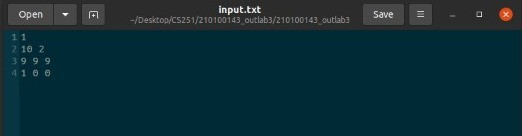
\includegraphics[width=\textwidth]{Q4_input.jpeg}
    \caption[]{Input}
\end{figure*}
\vspace*{2em}
\begin{figure*}[h]
    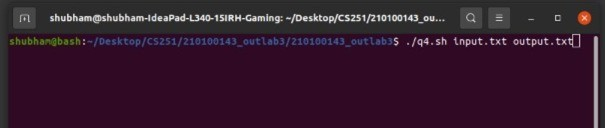
\includegraphics[width=\textwidth]{Q4_command.jpeg}
    \caption[]{Command}
\end{figure*}
\vspace*{2em}
\begin{figure*}[h]
    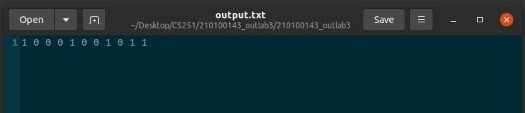
\includegraphics[width=\textwidth]{Q4_output.jpeg}
    \caption[]{Output}
\end{figure*}
\newpage

\bibliographystyle{plain}
\bibliography{mybibliography} 


\end{document}